\documentclass[a4paper]{article}

%% Language and font encodings
\usepackage[english]{babel}
\usepackage[utf8x]{inputenc}
\usepackage[T1]{fontenc}

%% Useful packages
\usepackage{amsmath}
\usepackage{graphicx}
\usepackage{hyperref}
\usepackage{enumitem}
\usepackage{mathtools}

\title{Marxian Economics TLDR}
\author{Socialism Done Left}

\begin{document}

\maketitle

This document briefly summarizes the main points of Marx's theory of capitalism.

\section{Commodities}

A \textbf{commodity} is any thing that has two qualities:

\begin{enumerate}
\item \textbf{exchange value} = the ability to be exchanged with another person
\item \textbf{use value} = the ability to be used for some purpose
\end{enumerate}

If you exchange a commodity, you cannot use it and its use value is 0 for you. Some commodities can be more easily exchanged and have greater exchange value: Coal in a pile is more difficult to exchange than coal in a bag.

If you use a commodity, you cannot exchange it and its exchange value is 0 for you. Some commodities can more easily achieve some purpose and have greater use value: A sharp axe can more easily achieve some purpose than a blunt axe.

Marx asserts that the value of a commodity comes from the labor put into it.

\section{Labor Theory of Value}
Marx's Labor Theory of Value (LTV) asserts that the price of production of a commodity will tend towards its average labor input.

\section{Profit}
Marx's theory of profit asserts that profit comes only from labor.

\[ \text{V'} = \text{VC} + \text{CC} + \text{SV} \]

\begin{itemize}
\item V' = latter Value = total ``value'' produced per production cycle
\item CC = Constant Capital = value of ``dead labor'' required per production cycle = machines, tools, electricity, materials, etc.
\item VC = Variable Capital = value of ``living labor'' required per production cycle = wages, benefits, etc.
\item SV = Surplus Value = V' - CC - VC = excess ``value'' added to the produced commodities per production cycle
\end{itemize}

The Rate of Profit (RoP) is profit per investment.

\[ \text{RoP} = \frac{\text{SV}}{\text{CC} + \text{VC}} \]

If you are a capitalist and you spend \$100 on wages (VC) and materials (MP) and you receive \$105 from sales, then you have a 5\% RoP.

\section{Circuit of capital}

Capital circulates from one form to another (metamorphoses) and increases in total value (valorizes) in a production cycle: An input capital ($C_{i,t}$) with an input value ($V_{i,t}$) is used to produce ($...P_{t}...$) an output capital ($C_{i,t}$) with an output value ($V_{o,t}$) for a value change of ($V_{o,t}-V_{i,t}=V'=SV$). Repeat.

\[
\text{cycle t-1}
\rightarrow
\underbrace{
	M_{t}
	\rightarrow
	\overbrace{
		C_{i,t}
	}^\text{$V_{i,t}$}
	\rightarrow
	...P_t...
	\rightarrow
	\overbrace{
		C_{o,t}
	}^{V_{o,t}}
}_\text{cycle t}
\rightarrow
\text{cycle t+1} \]

\begin{itemize}
\item {$M_{t}$ = money form = money from sales used to obtain MP and LP}
\item {$C_{i,t}$ = input capital form = purchased commodities (MP, LP) used to obtain produced commodities}
\begin{itemize}
\item {[M]eans of [P]roduction: produced commodities that enable production of other produced commodities}
\item {[L]abor [P]ower = labor}
\end{itemize}
\item {[P]roduction form = in which LP acts upon MP to produce surplus value in the forms of new consumption goods and new means of production}
\item {[O]utput [C]ommodity form = produced commodities (MP, CG, LG) used to obtain money from sales}
\begin{itemize}
\item {[M]eans of [P]roduction = commodities purchased to enable production of other commodities, to be sold on a MP market}
\item {[A]rticles of [G]onsumption = commodities produced for essential human consumption, to be sold on a CG market}
\item {[N]onessential [G]oods = commodities produced for non-essential consumption, to be sold on a CG market}
\end{itemize}
\end{itemize}

RoSV = Rate of Surplus Value = value of surplus value per value of variable capital = profit per worker

\[ \text{RoSV} = \frac{\text{SV}}{\text{VC}} \]

RoCCtVC = Ratio of Constant Capital to Variable Capital = value of constant capital per value of variable capital = machines(*) per worker

\[ \text{RoCCtVC} = \frac{\text{SV}}{\text{VC}} \]

\section{Marx's law of the tendency of the rate of profit to fall:}

If we multiply the RoP equation by a factor equal to one, we derive a useful relationship:

\[ \text{RoP} \times \frac{\frac{1}{\text{VC}}}{\frac{1}{\text{VC}}} = \frac{\frac{\text{SV}}{\text{VC}}}{\frac{\text{CC}}{\text{VC}} + \frac{\text{VC}}{\text{VC}}}  = \frac{\text{RoSV}}{\text{RoCCtVC} + 1} \]

If RoSV rises more slowly than RoCCtVC, then RoP will converge to 0. If RoCCtVC rises more slowly than RoSV, then RoP will converge infinitely upward. Thus, the question becomes which rate increases faster? A quote from \href{https://content.csbs.utah.edu/~mli/Economics\%207004/Basu-tendency\%20for\%20the\%20rate\%20of\%20profit\%20to\%20fall.pdf}{Basu 2012} explains why RoP is likely to decline:

\begin{quote}
This increasing mechanization of the production process enormously increases the productivity of labor and facilitates the extraction of larger amounts of relative surplus value. The increasing replacement of labor with non-labor inputs is reflected in a rise of the share of total capital outlays supporting constant capital in relation to variable capital. Consequently, what Marx called the organic composition of capital rises and there is a reduction in the amount of labor available for exploitation by capital per unit of capital outlay. If the rate of surplus value remains constant, this fall in the composition of capital can lead to a fall in the rate of profit.
\end{quote}

\section{Empirical data:}

Analysis from \href{https://content.csbs.utah.edu/~mli/Renmin\%20Summer\%202017/Maito-MPRA_paper_55894.pdf}{Maito 2014} suggests that the rate of profit in the core countries (the United States, the United Kingdom, Japan, Germany, the Netherlands, and Sweden) has declined for the past century and a half, from about 40\% in 1869 to about 12.5\% in 2010:

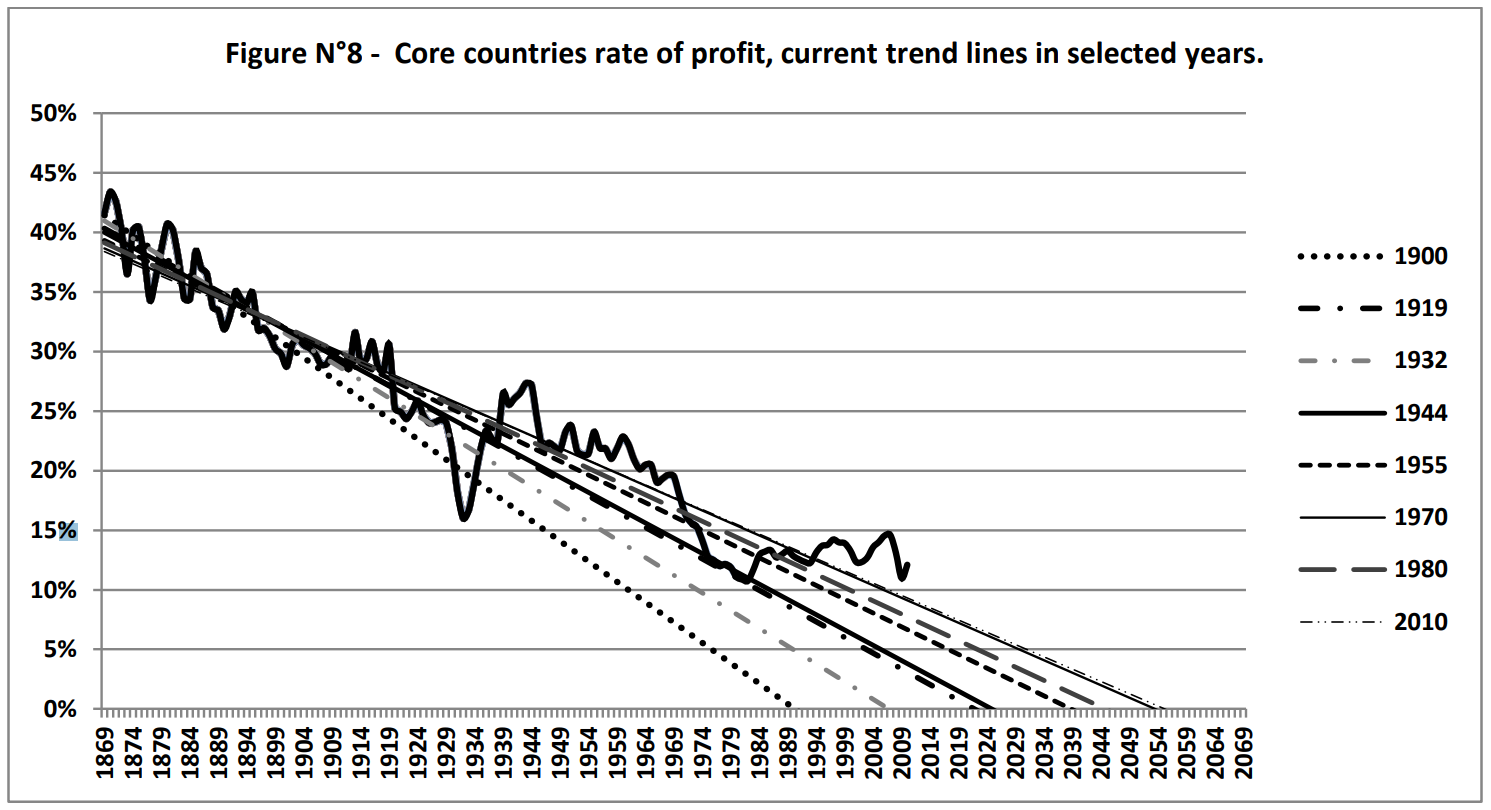
\includegraphics[width=\textwidth]{maito}

The year that RoP is projected to hit zero ($\text{RoP}_0$) has moved forward over the years; however, this movement has not kept pace with time itself. In the past 110 years, the number of years until $\text{RoP}_0$ has been cut in half: from 89 years to 46 years:

\begin{center}
\begin{tabular}{ r | l | l }
\hline
Year & $\text{RoP}_0$ & $\text{RoP}_0$ - Year \\
\hline
1900 & 1989 & 89 \\
1919 & 2022 & 93 \\
1932 & 2004 & 72 \\
1944 & 2024 & 80 \\
1955 & 2039 & 84 \\
1970 & 2051 & 45 \\
1980 & 2043 & 63 \\
2010 & 2056 & 46 \\
\hline
\end{tabular}
\end{center}

\section{Conclusions:}

If the RoP is genuinely falling, as it appears to be, then capitalism's years are limited.

\end{document}

$C_{t}$ is composed of human-related costs, such as wages and healthcare -- variable capital (VC) -- and non-human-related costs, such as materials and machines -- constant capital (CC).
